\documentclass[border=10pt]{standalone}
\usepackage[svgnames]{xcolor}
\usepackage{amsmath}
\usepackage{pgfplots}
\pgfplotsset{compat=newest}
\usepackage[sfdefault]{FiraSans}
\usepackage{FiraMono}
\renewcommand*\familydefault{\sfdefault}
\begin{document}
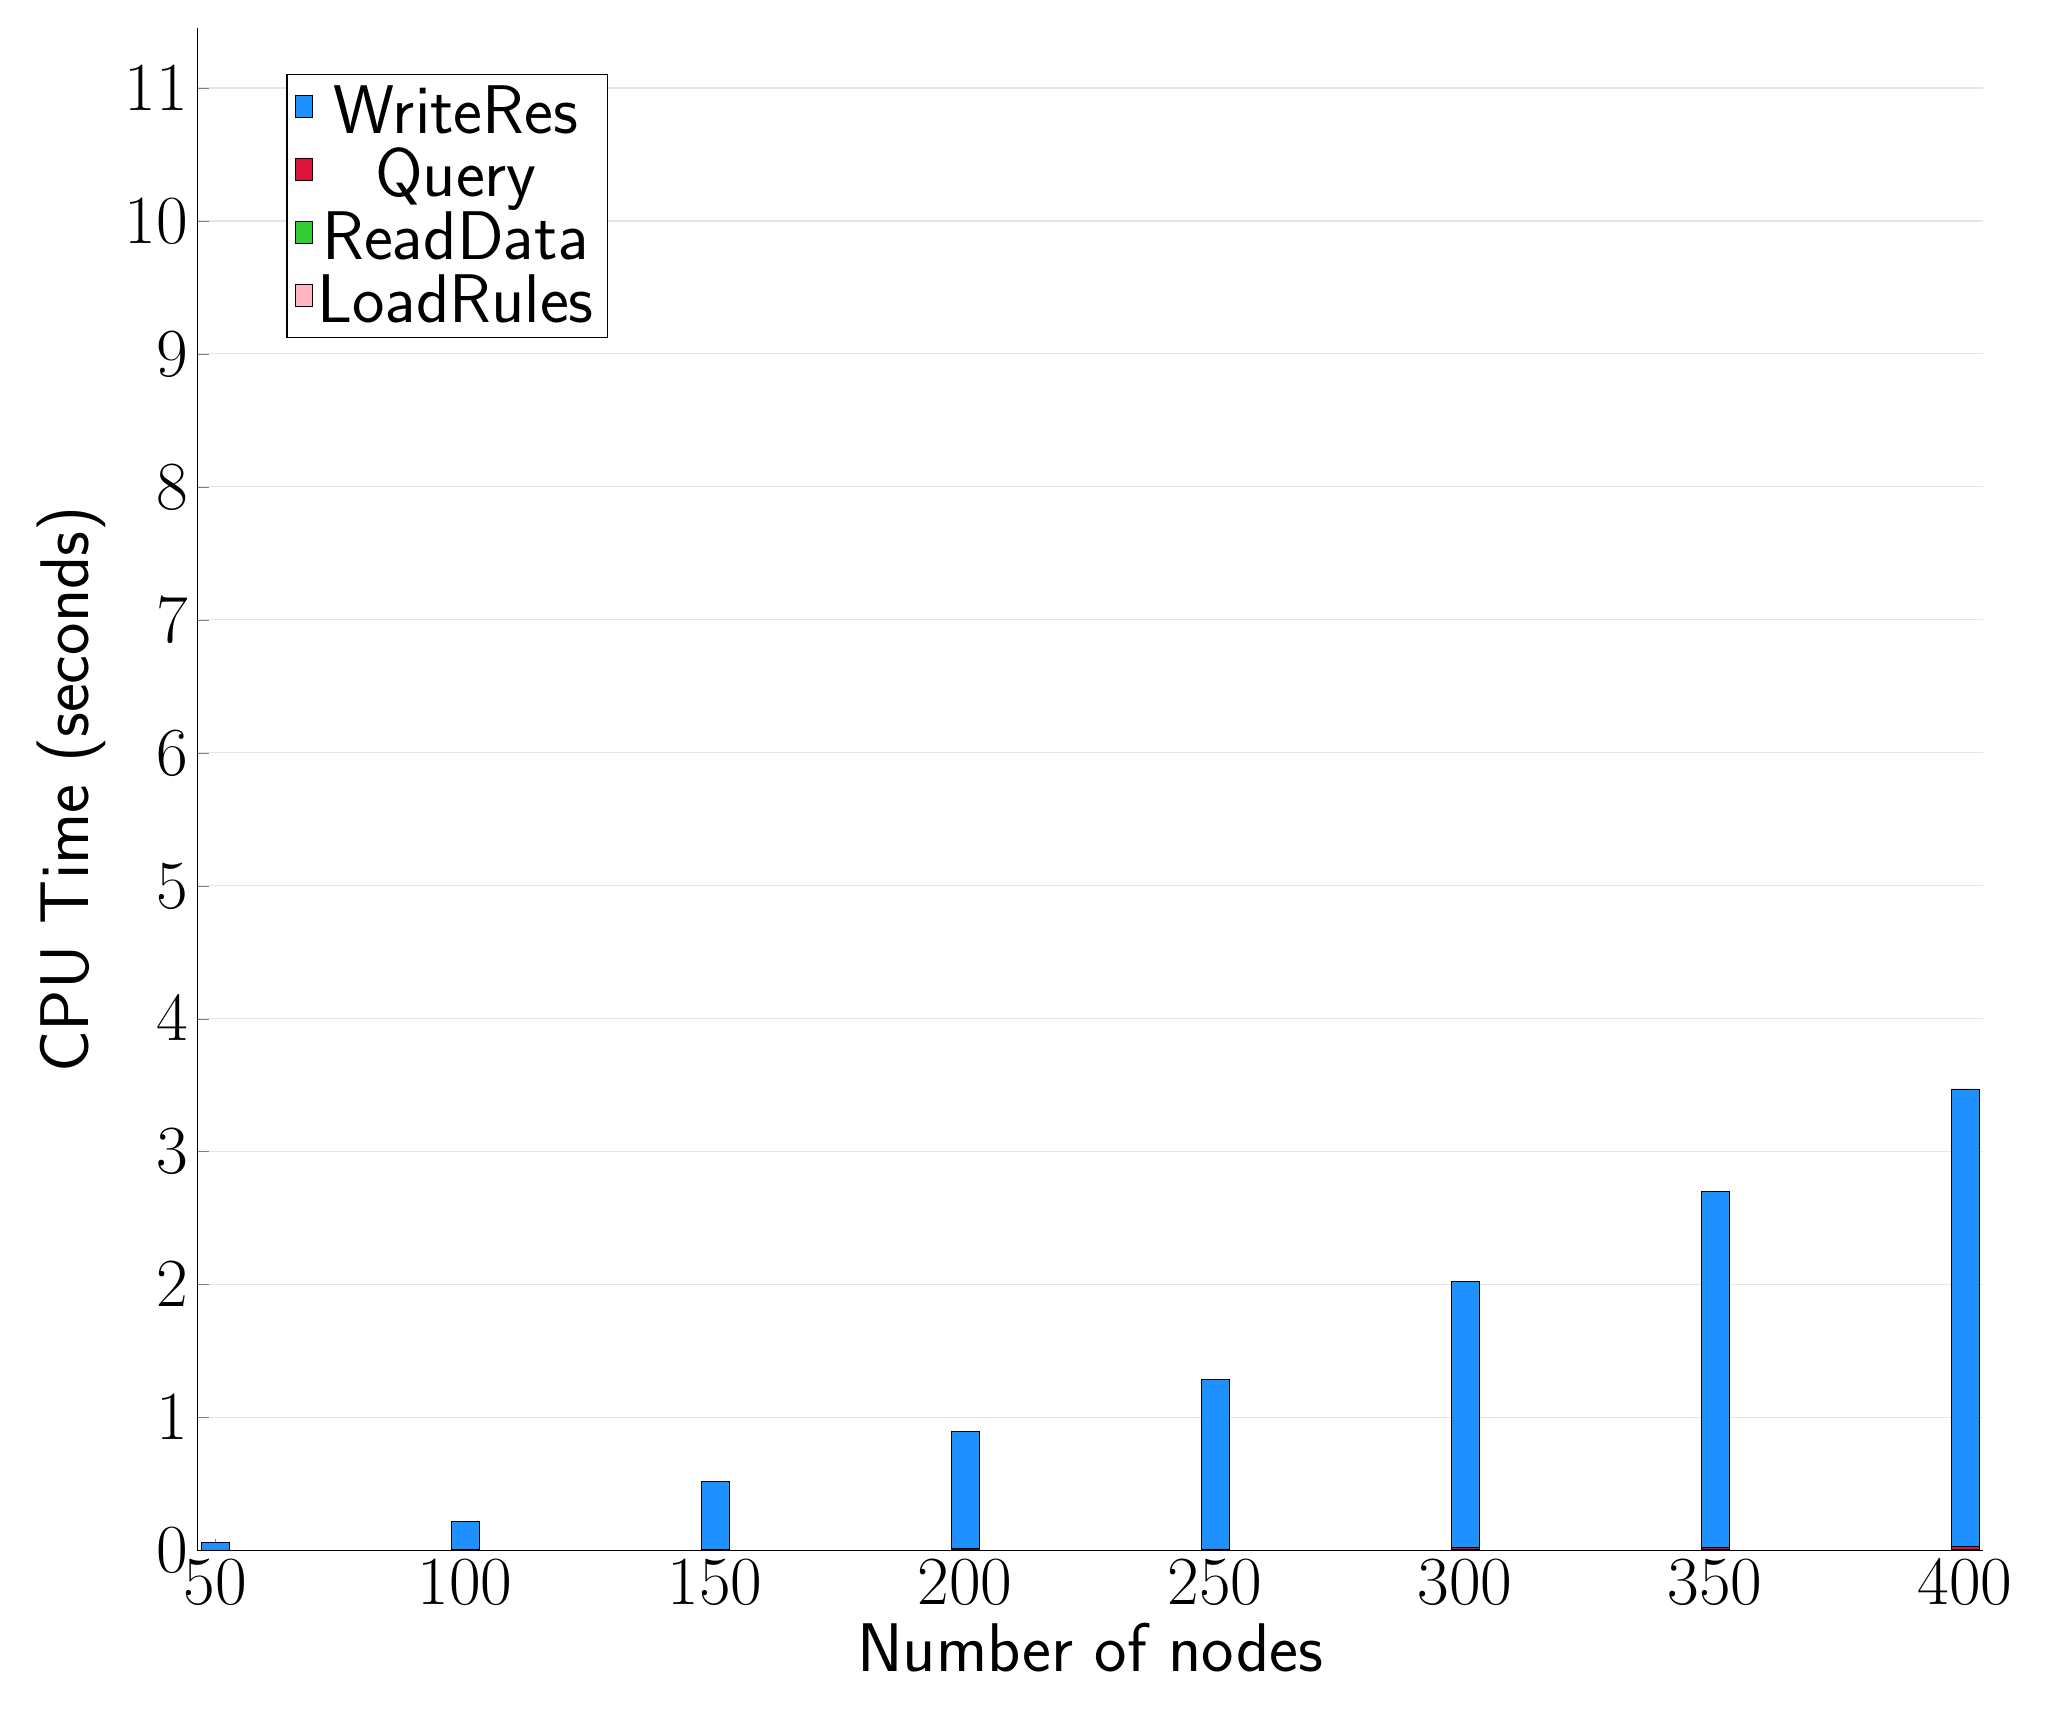
\begin{tikzpicture}
\begin{axis}[
   ybar stacked,
   width=2\textwidth,
   bar width=0.35cm,
   ymajorgrids, tick align=inside,
   major grid style={draw=gray!20},
   xtick=data,
   ymin=0, ymax=11.449559211730957,
   axis x line*=bottom,
   axis y line*=left,
   enlarge x limits=0.01,
   legend style={
       at={(0.23, 0.97)},
       anchor=north east,
       legend columns=1,
       font=\Huge,
   },
   ylabel={CPU Time (seconds)},
   xlabel={Number of nodes},
   label style={font=\Huge},
   tick label style={font=\Huge},
]
\addlegendimage{fill=DodgerBlue, draw=black, line width=0.2pt}
\addlegendentry{WriteRes}
\addlegendimage{fill=Crimson, draw=black, line width=0.2pt}
\addlegendentry{Query}
\addlegendimage{fill=LimeGreen, draw=black, line width=0.2pt}
\addlegendentry{ReadData}
\addlegendimage{fill=LightPink, draw=black, line width=0.2pt}
\addlegendentry{LoadRules}
\addplot +[fill=LightPink, draw=black, line width=0.2pt] coordinates {
(50, 0.0040120000000000025)
(100, 0.00481366666666667)
(150, 0.004752333333333333)
(200, 0.005040333333333337)
(250, 0.003108666666666667)
(300, 0.00389433333333334)
(350, 0.0037883333333333332)
(400, 0.0033330000000000005)
};
\addplot +[fill=LimeGreen, draw=black, line width=0.2pt] coordinates {
(50, 0.0016073333333333235)
(100, 0.0023743333333333333)
(150, 0.0036070000000000065)
(200, 0.004365000000000001)
(250, 0.003822333333333334)
(300, 0.0050683333333333335)
(350, 0.005576666666666667)
(400, 0.004511999999999999)
};
\addplot +[fill=Crimson, draw=black, line width=0.2pt] coordinates {
(50, 0.0003023333333333327)
(100, 0.001279333333333327)
(150, 0.0035156666666666635)
(200, 0.006404333333333337)
(250, 0.007226999999999997)
(300, 0.012758)
(350, 0.014266666666666669)
(400, 0.024838666666666665)
};
\addplot +[fill=DodgerBlue, draw=black, line width=0.2pt] coordinates {
(50, 0.053944)
(100, 0.21452433333333334)
(150, 0.5101436666666667)
(200, 0.8802796666666667)
(250, 1.2762033333333334)
(300, 2.0020466666666668)
(350, 2.6777953333333335)
(400, 3.440412333333333)
};
\end{axis}
\end{tikzpicture}

\end{document}
